\documentclass[a4paper]{article}

% CJK support: prefer ctex, fallback to XeTeX native line breaking
\IfFileExists{ctex.sty}{
  \usepackage[fontset=fandol]{ctex}
}{
  % Fallback for minimal TeX installs (e.g. MacTeX Basic, TeX Live scheme-basic)
  % without ctex/xeCJK. Uses XeTeX's built-in CJK line breaking.
  \usepackage{fontspec}
  \XeTeXlinebreaklocale "zh"
  \XeTeXlinebreakskip = 0pt plus 1pt
  \IfFontExistsTF{Songti SC}{\setmainfont{Songti SC}}{%
    \IfFontExistsTF{Noto Serif CJK SC}{\setmainfont{Noto Serif CJK SC}}{}%
  }
  \IfFontExistsTF{Heiti SC}{\setsansfont{Heiti SC}}{%
    \IfFontExistsTF{Noto Sans CJK SC}{\setsansfont{Noto Sans CJK SC}}{}%
  }
}

% Basic packages
\usepackage{amsmath, amssymb}
\usepackage{graphicx}
\usepackage[margin=2.5cm]{geometry}
\emergencystretch=3em
\usepackage[most]{tcolorbox}
\usepackage{etoolbox}
\usepackage{listings}
\usepackage{hyperref}
\usepackage{booktabs}
\usepackage{array}
\usepackage{subcaption}
\usepackage{float}
\usepackage{tikz}
\IfFileExists{pgfplots.sty}{
    \usepackage{pgfplots}
    \pgfplotsset{compat=1.18}
}{}

% ===== Highlight boxes =====
\newtcolorbox{knowledgebox}[1]{
    enhanced, colback=blue!5!white, colframe=blue!75!black, colbacktitle=blue!75!black,
    coltitle=white, fonttitle=\bfseries, title={#1}, attach boxed title to top left={yshift=-2mm, xshift=2mm},
    boxrule=1pt, sharp corners
}

\newtcolorbox{importantbox}[1]{
    enhanced, colback=yellow!10!white, colframe=yellow!80!black, colbacktitle=yellow!80!black,
    coltitle=black, fonttitle=\bfseries, title={#1}, sharp corners
}

\newtcolorbox{warningbox}[1]{
    enhanced, colback=red!5!white, colframe=red!75!black, colbacktitle=red!75!black,
    coltitle=white, fonttitle=\bfseries, title={#1}, sharp corners
}

\newtcolorbox{practicebox}[1]{
    enhanced, colback=black!3!white, colframe=black!75, colbacktitle=black!75,
    coltitle=white, fonttitle=\bfseries, title={#1}, sharp corners
}

% ===== Code listings =====
\lstset{
    basicstyle=\ttfamily\small,
    keywordstyle=\color{blue},
    stringstyle=\color{red!60!black},
    commentstyle=\color{green!60!black},
    breaklines=true,
    frame=single,
    numbers=left,
    numberstyle=\tiny\color{gray},
    captionpos=b,
    extendedchars=false
}

% ===== Figure provenance and unit macros =====
% \vtag goes inside \caption{...}; \srcnote{MM:SS--MM:SS} follows the figure environment.
\newcommand{\vtag}{\protect\footnotemark}
\newcommand{\srcnote}[1]{\footnotetext{视频画面时间区间：#1。若为裁剪图，时间区间仍对应原视频画面。}}
% Units work in text and math mode; never hand-write $^\circ$ or \AA inside \mathrm.
\newcommand{\degC}{\ensuremath{^{\circ}\mathrm{C}}}
\newcommand{\um}{\ensuremath{\mu\mathrm{m}}}
\newcommand{\nm}{\ensuremath{\mathrm{nm}}}
\newcommand{\angstrom}{\ensuremath{\text{\AA}}}

% ===== Front-page metadata =====
% Fill these in when generating notes.
\newcommand{\notetitle}{智能体编程}
\newcommand{\notesubtitle}{MIT Missing Semester 2026 · 第 7 讲：编码智能体的原理、用例与上下文管理}
\newcommand{\noteauthors}{根据 MIT Missing Semester 2026 课堂录像整理（Anish 主讲）}
\newcommand{\notedate}{2026年1月21日（课堂）}
\newcommand{\videochannel}{Missing Semester（YouTube）}
\newcommand{\videopublishdate}{2026年}
\newcommand{\videoduration}{1小时0分34秒}
\newcommand{\videourl}{https://www.youtube.com/watch?v=sTdz6PZoAnw}
\newcommand{\videocoverpath}{cover.jpg}

\setlength{\emergencystretch}{3em}
\begin{document}

% ===== Title page =====
\begin{titlepage}
\centering
{\Large 课程笔记\par}
\vspace{1.2cm}
{\huge\bfseries \notetitle\par}
\ifdefempty{\notesubtitle}{}{
\vspace{0.3cm}
{\large \notesubtitle\par}
}
\vspace{0.5cm}
{\large \noteauthors\par}
\vspace{0.3cm}
{\large \notedate\par}
\vspace{1.0cm}

\ifdefempty{\videocoverpath}{
{\small 请在生成笔记时填入视频封面图的本地路径。\par}
}{
\includegraphics[width=0.82\textwidth,height=0.40\textheight,keepaspectratio]{\videocoverpath}\par
}

\vfill
\begin{tcolorbox}[width=0.9\textwidth, colback=black!2!white, colframe=black!60, sharp corners]
\textbf{视频作者/频道}：\videochannel\par
\textbf{发布日期}：\videopublishdate\par
\textbf{视频时长}：\videoduration\par
\textbf{视频链接}：
\ifdefempty{\videourl}{
未填写
}{
\href{\videourl}{\nolinkurl{\videourl}}
}
\end{tcolorbox}
\end{titlepage}

\tableofcontents
\newpage

%% --- 正文内容开始 --- %%

\section{这一讲讲什么}

这是 Missing Semester 的第七天，主题是智能体编程（agentic coding），延续上周“开发环境与工具”一讲中 AI 辅助开发的话题。讲者 Anish 回顾：上次讲了自动补全和行内聊天这类 AI 辅助编程；今天要讲的是更复杂、更新的东西，一种与五年前存在的工具都不同的形态：编码智能体（coding agent）。他计划先演示这些工具怎样工作，再讲它们在底层怎样实现，最后讲用例和进阶功能。

\begin{knowledgebox}{本讲结构}
讲义作者整理：第一部分用 Claude Code 演示一个端到端的任务；第二部分在黑板上从语言模型、多轮对话、工具调用一步步搭出“智能体框架”的概念；第三部分讲用例，包括修 bug、代码审查、理解代码库、当作 Shell 使用和氛围编程；第四部分讲进阶功能，包括可复用提示词、并行智能体与 git worktree、MCP，以及一系列上下文管理手段。
\end{knowledgebox}

\section{第一个演示}

\subsection{把脚本变成命令行程序}

\noindent\begin{minipage}{\textwidth}
\begin{figure}[H]
\centering
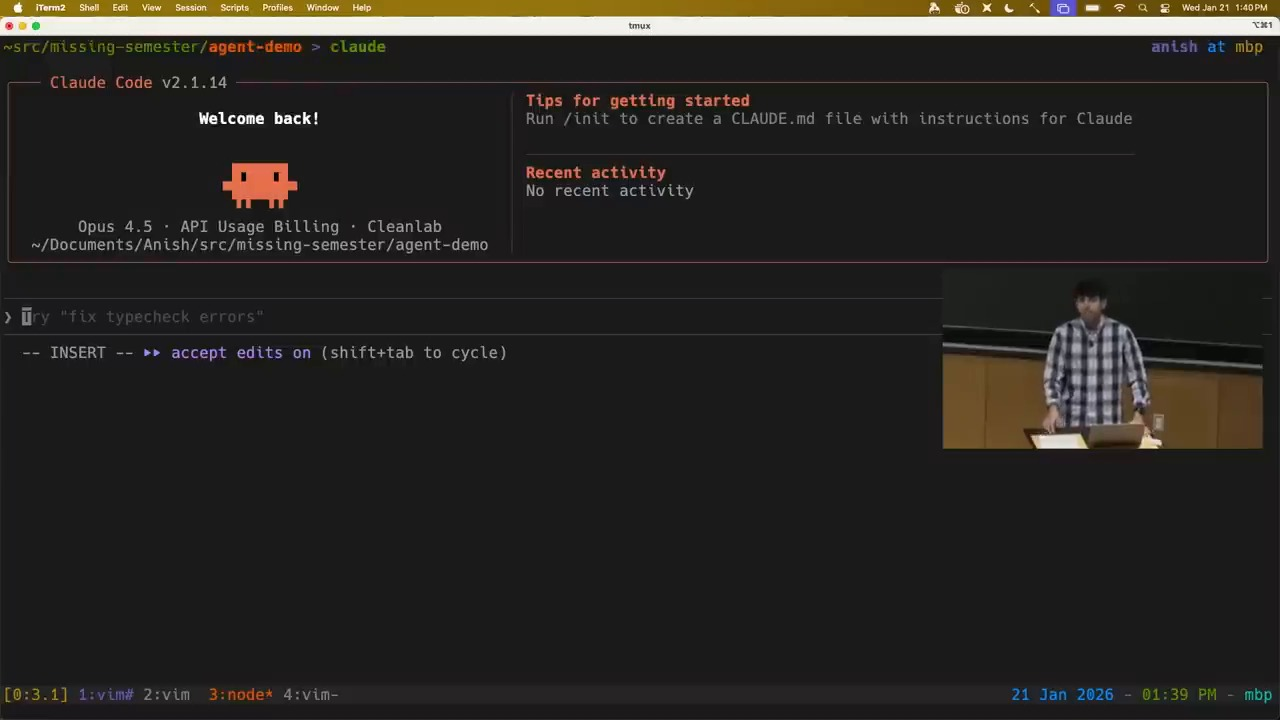
\includegraphics[width=0.92\textwidth]{figures/fig_01_claude_start.jpg}
\caption{在代码目录中输入 claude 启动 Claude Code 的命令行界面\vtag}
\end{figure}
\srcnote{00:02:30--00:02:45}
\end{minipage}


讲者回顾上次写的那个小 Python 脚本：从课程网站下载一个页面并提取其中所有链接。假设想把这个拼凑出来的脚本变成一个更像样的命令行程序，比如加上参数解析，把要抓取的页面变成命令行参数，就可以让编码智能体端到端地完成整个任务。他说有好几种命令行编码智能体，比如 Claude Code 和 Codex，他个人目前更喜欢用命令行形式的；VS Code、Cursor 等 IDE 里也内置了大致相同的功能。他在代码所在目录打开终端，输入 \texttt{claude}，就打开了 Claude Code 的命令行界面。

讲者解释，编码智能体基本上就是一个对话式 AI 模型，再加上一些帮助它写代码的工具。如果用过 ChatGPT，这大致就是 ChatGPT，只不过 AI 模型可以在你的电脑上做事：读写文件、运行命令等。

他输入了自然语言指令（故意留着一个拼写错误）：把我写的脚本 \texttt{dl.py} 变成一个正经的命令行程序，用 \texttt{argparse} 做参数解析；确保有正确的类型注解，并用 mypy 检查它能通过类型检查。

\noindent\begin{minipage}{\textwidth}
\begin{figure}[H]
\centering
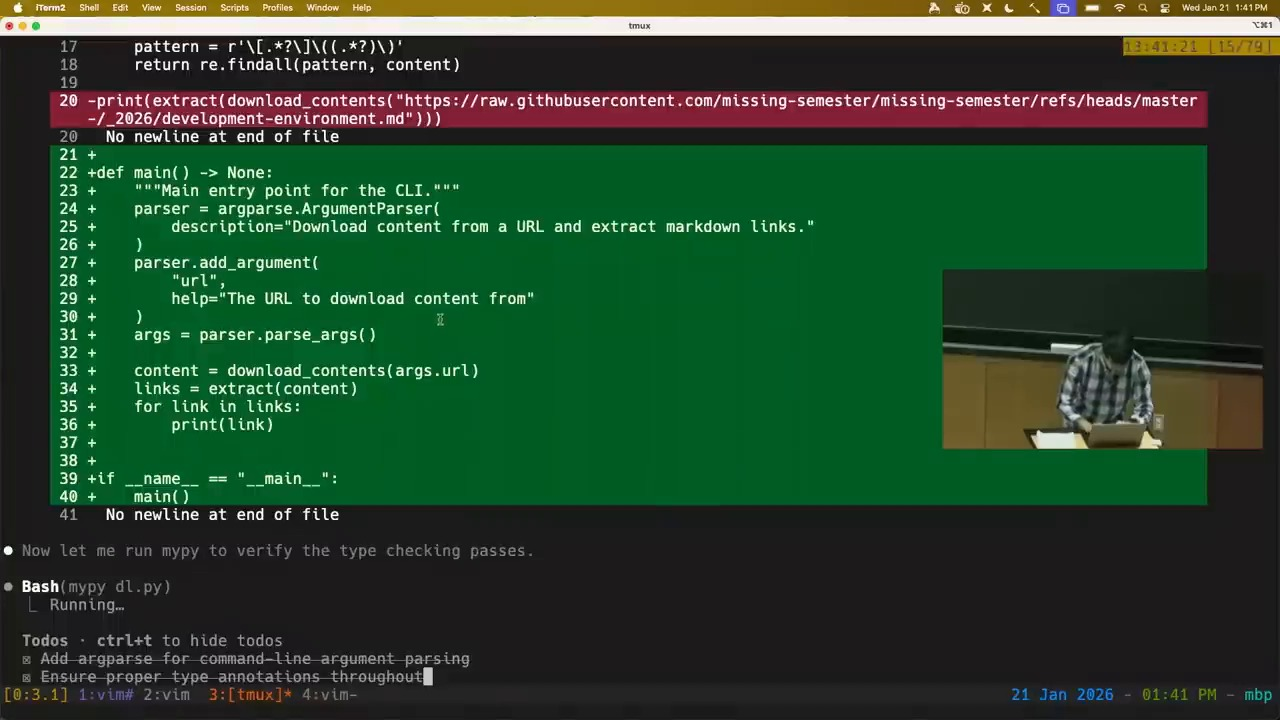
\includegraphics[width=0.92\textwidth]{figures/fig_02_diff_review.jpg}
\caption{智能体一次性改写了 dl.py，红绿差异显示新增的函数和 main 中的参数解析\vtag}
\end{figure}
\srcnote{00:04:15--00:04:30}
\end{minipage}


这是一个很简单的任务，智能体更新了 \texttt{dl.py}，一次性写好了所有代码。可以看到它写了更多函数，现在有一个包含命令行参数解析的 \texttt{main} 函数。它完成了要求的整个任务，并且继续遵循指令：记得他要求有类型注解并通过类型检查，于是它接下来要调用 Shell，运行 mypy 并把脚本路径作为参数。

\subsection{逐个批准工具调用}

\noindent\begin{minipage}{\textwidth}
\begin{figure}[H]
\centering
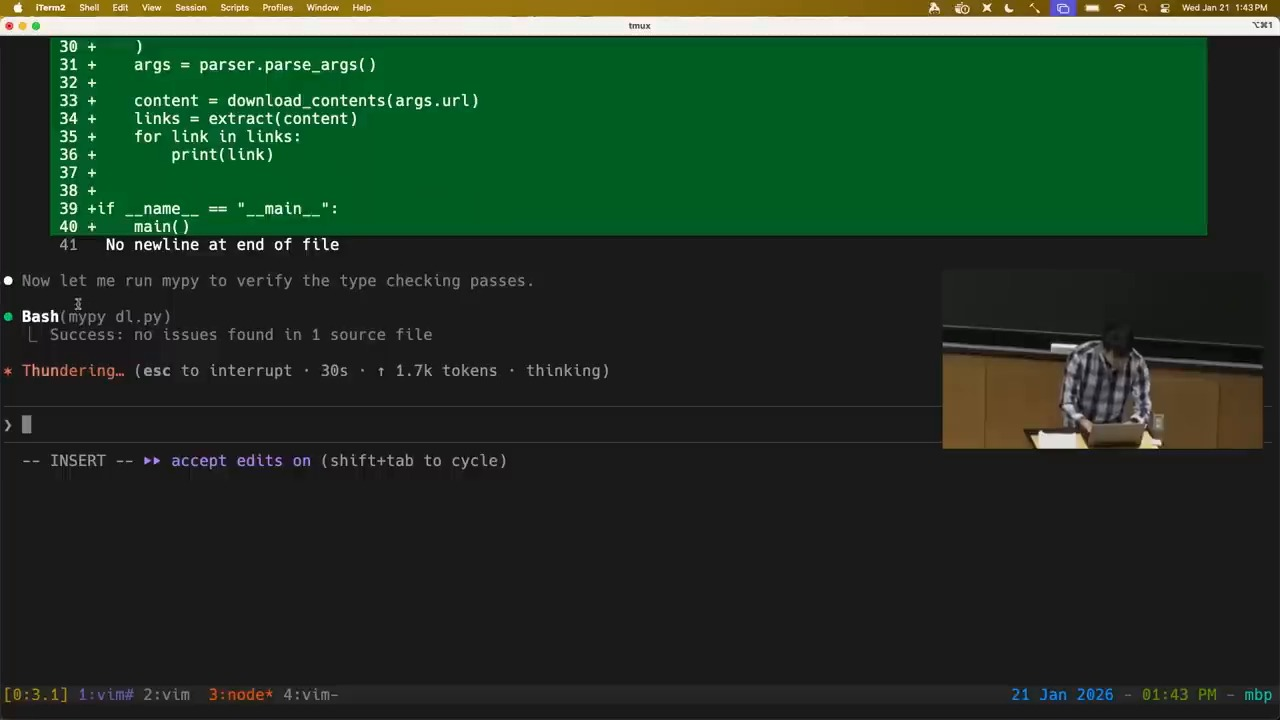
\includegraphics[width=0.92\textwidth]{figures/fig_03_mypy_approve.jpg}
\caption{智能体请求运行 mypy 时停下来等待批准\vtag}
\end{figure}
\srcnote{00:05:30--00:05:45}
\end{minipage}


讲者注意到，智能体修改文件时没有逐一请他批准，而运行 bash 命令时却停下来等他确认。他说这是他对这个工具的配置：文件修改可以让智能体先做一堆，之后一次性审查；但像 bash 这样的工具，他想检查智能体运行的每一条命令，确保它是安全的。

\begin{warningbox}{不要让智能体完全自主运行}
讲者说今天不深入智能体安全，但如果让它们完全自主运行，确实存在安全隐患：它们可能调用你不希望运行的命令，比如删除你在乎的文件，或者做比这危险得多的事。他个人建议在需要逐个批准工具调用的模式下运行它们。
\end{warningbox}

\noindent\begin{minipage}{\textwidth}
\begin{figure}[H]
\centering
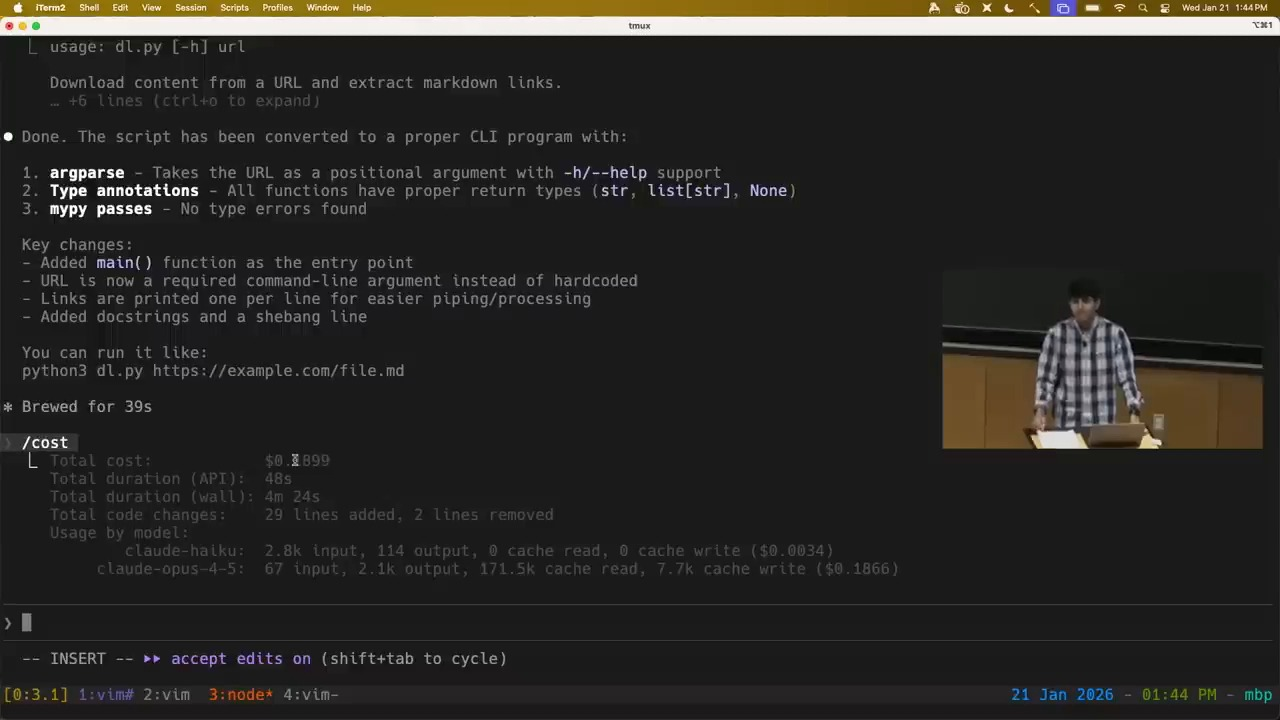
\includegraphics[width=0.92\textwidth]{figures/fig_04_done_summary.jpg}
\caption{mypy 通过后，智能体总结了它所做的修改并把控制权交还给用户\vtag}
\end{figure}
\srcnote{00:07:00--00:07:15}
\end{minipage}


mypy 运行通过，智能体给出了总结：添加了 \texttt{argparse}、类型注解、通过了类型检查等。

\subsection{费用与离线使用}

有同学问：这在后台使用托管的 AI 服务，能否限制花多少钱？讲者说可以，具体配置因工具而异。一般可以选择用哪个模型，能力更强、更擅长难任务的模型更贵，更小更快的模型更便宜；有些服务还能设置消费上限，比如每月最多 10 美元。他建议学生可以从每月 20 美元左右的订阅计划开始，里面包含一定的用量；超出时再想想自己是怎样使用 AI 的。他知道在很多公司，工程师很喜欢这些工具，生产力提升足够大，与工程师的时间成本相比，工具费用相对较低，所以很多人每月在 AI 上花几百美元也没问题。

有同学问编码智能体是否需要联网。讲者说基本需要：离线的话只能使用能力弱得多的模型，简单任务也许还行，难一点的就不太行了，目前实际可行的是使用托管模型并付费。至于订阅还是一次性付费，他说基本都是订阅，因为推理成本取决于用量；定价模式各不相同，可以自己去查，这一讲不想花太多时间在定价上。

\begin{knowledgebox}{常见的编码智能体形态}
讲义作者补充：编码智能体大致有三种形态：命令行智能体（如讲者演示的 Claude Code，以及 Codex CLI、开源的 OpenCode 等），IDE 内置的智能体面板（如 VS Code 的 Copilot 智能体模式、Cursor），以及在云端运行、直接提交拉取请求的后台智能体。它们共享同一套原理：语言模型加智能体框架加工具。
\end{knowledgebox}

\subsection{多轮交互与反馈循环}

\noindent\begin{minipage}{\textwidth}
\begin{figure}[H]
\centering
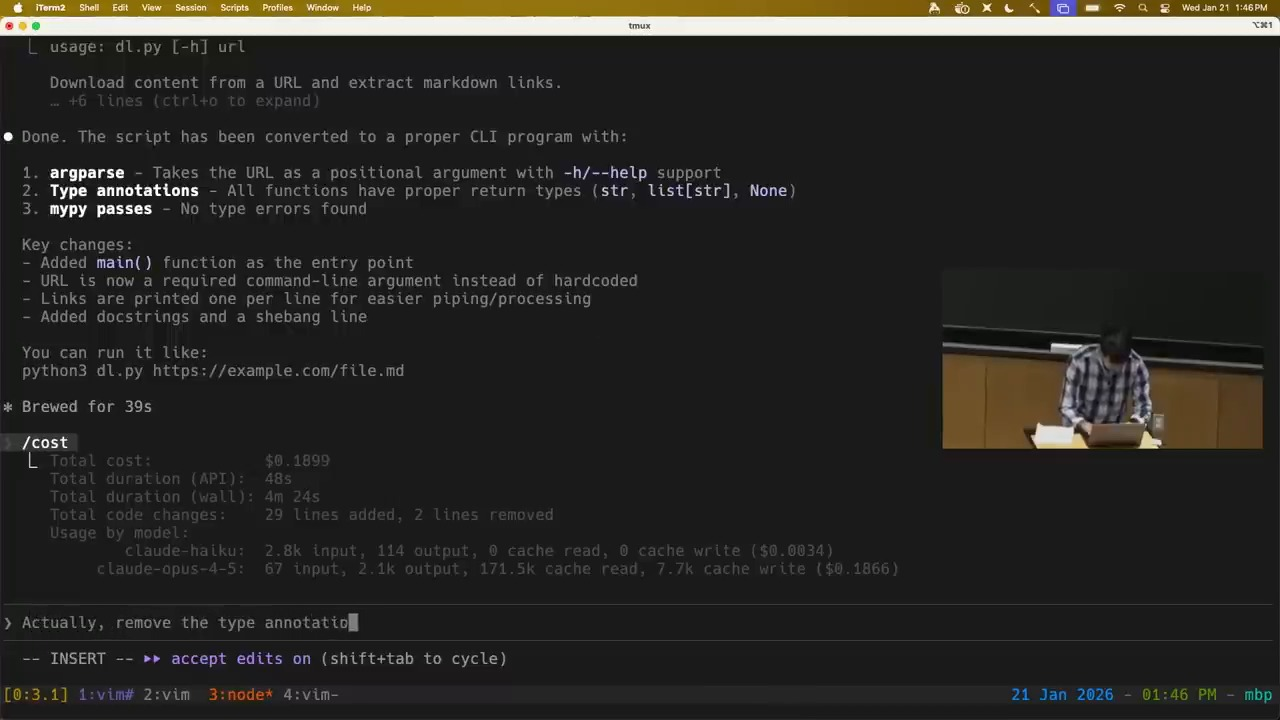
\includegraphics[width=0.92\textwidth]{figures/fig_05_multiturn.jpg}
\caption{在同一会话中追加一条消息，要求去掉类型注解，智能体沿用之前的上下文继续修改\vtag}
\end{figure}
\srcnote{00:09:00--00:09:15}
\end{minipage}


也可以和智能体多轮交互。讲者让它去掉类型注解，它会继续工作，因为它有之前对话的上下文。他承认这很傻，让程序变差了，但它照做了。更实际的用法是在正在做的东西上迭代：做一个规格还不完全清楚的功能时，给它一个粗略描述，它做出来，你评判结果，再说“其实我想让你这样或那样调整”。还可以告诉它环境的细节，比如“mypy 在这里，这样调用它”。

有同学问能否硬性规定“不要动这个文件或这部分代码”。讲者说在他用的工具里，不能硬性禁止修改文件的某个部分。他实际的做法是用 Git 跟踪一切，看它改了什么，改了不想改的就还原；也可以给自然语言指令，比如“除了这个函数，去掉所有类型注解”或“不要改这一段”。

\begin{importantbox}{让智能体在反馈循环中工作}
讲者说，测试驱动开发是使用这些工具的好方法：要么自己写测试，再让智能体实现功能使测试通过；要么先让智能体帮你写测试，再让它实现通过测试的功能。这些工具在有反馈循环时效果很好：代码编译不过、类型检查不过时，告诉它“这是错误，这样运行可以复现，一直改到修好为止”。
\end{importantbox}

\section{编码智能体怎样工作}

讲者说，这个话题可以讲整整一学期，但他会尽量停在合适的抽象层次上，让大家学到有效使用这些工具所需的部分。他不会教大家怎样自己重新实现一个，但会讲一点它们的工作原理，让大家理解它们擅长什么、有什么局限，以及为什么人们在智能体框架中实现了某些功能。他把 AI 编码智能体大致分为两个主要部分：底层的语言模型，以及包在语言模型外面的智能体框架（agent harness）。

\subsection{语言模型：条件概率分布}

\noindent\begin{minipage}{\textwidth}
\begin{figure}[H]
\centering
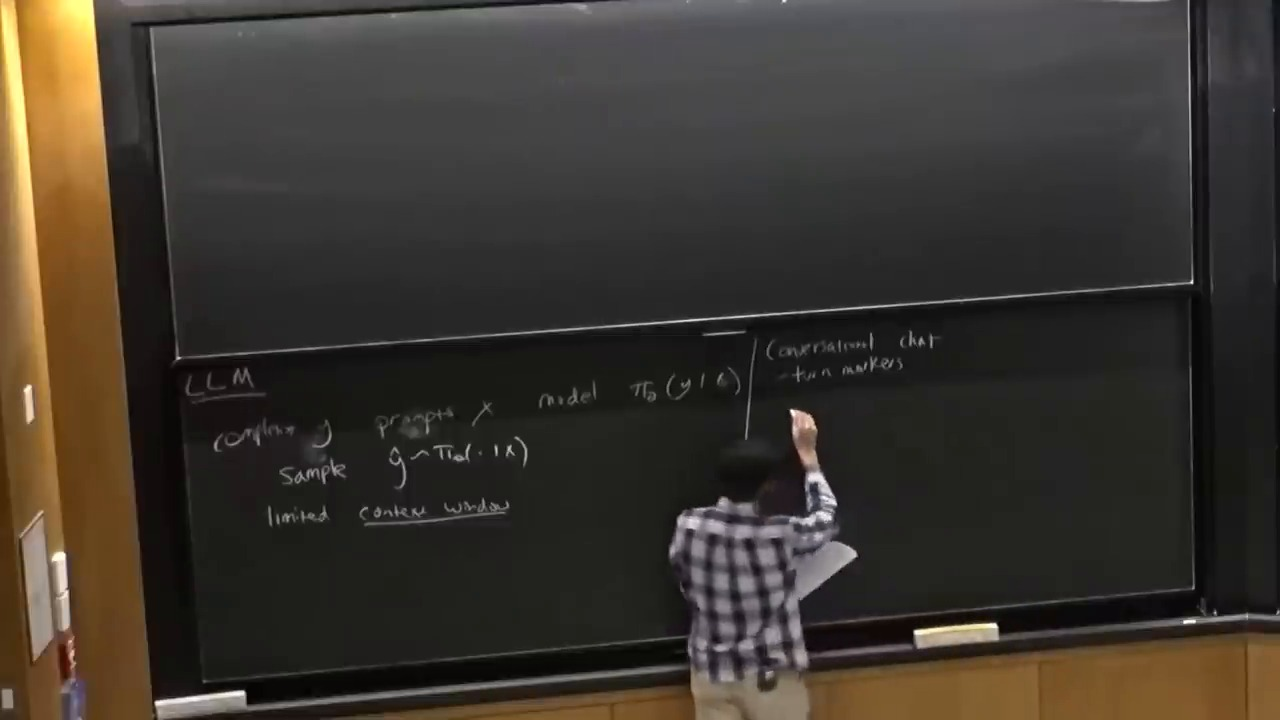
\includegraphics[width=0.92\textwidth]{figures/fig_06_llm_board.jpg}
\caption{黑板上的定义：语言模型是给定提示 x 时补全 y 的概率分布\vtag}
\end{figure}
\srcnote{00:15:30--00:15:45}
\end{minipage}


语言模型，有时叫大语言模型，可以看作在给定提示字符串 $x$ 的条件下，对补全字符串 $y$ 的概率分布建模。也就是一个条件生成模型：给定一个输入序列，告诉我们对应的输出字符串的概率分布。讲者把这个参数化的分布写作
\[
  y \sim \pi_\theta(y \mid x),
\]
其中 $\theta$ 是模型参数。他说，AI 语言模型就是这样，仅此而已。找到一个能做有用事情的好分布需要大量工作，但实际使用时就是给它一些文本（字符串或 token）作为输入，它返回一些文本作为输出，其余一切都建立在这个核心原语之上。另一个细节是：实践中它们的上下文窗口有限，即输入字符串和输出字符串的长度都有上限。

\subsection{多轮对话}

\noindent\begin{minipage}{\textwidth}
\begin{figure}[H]
\centering
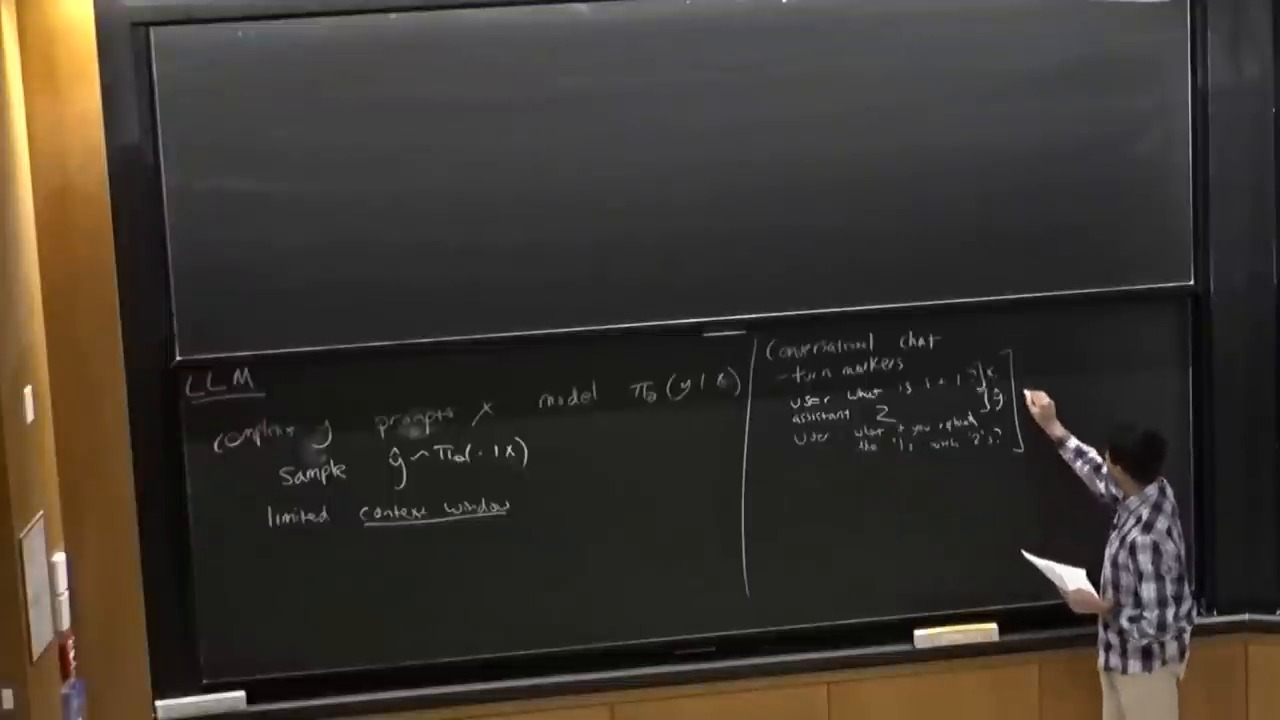
\includegraphics[width=0.92\textwidth]{figures/fig_07_chat_board.jpg}
\caption{多轮对话：把带轮次标记的整段对话历史作为下一次的提示\vtag}
\end{figure}
\srcnote{00:16:30--00:16:45}
\end{minipage}


在此基础上，ChatGPT 这样的东西怎样工作？单轮对话不难想象：问题作为输入，答案作为输出。那追问怎么办？讲者说，它们使用轮次标记（turn markers），把整段对话历史作为模型的输入，模型给出下一段输出。比如输入“用户：1 加 1 等于几？”，第一次采样时模型输出“助手：2”。然后追问一个依赖上下文的问题：“如果把 1 换成 2 呢？”这个问题单独看没什么意义，需要上下文才能正确回答。对话应用的处理方式是：把整段内容，用特殊编码的轮次标记分隔（用户说了这个，模型输出了那个，现在用户又说了这个），作为提示再次从语言模型采样，得到下一个输出。

\subsection{工具调用与智能体框架}

\noindent\begin{minipage}{\textwidth}
\begin{figure}[H]
\centering
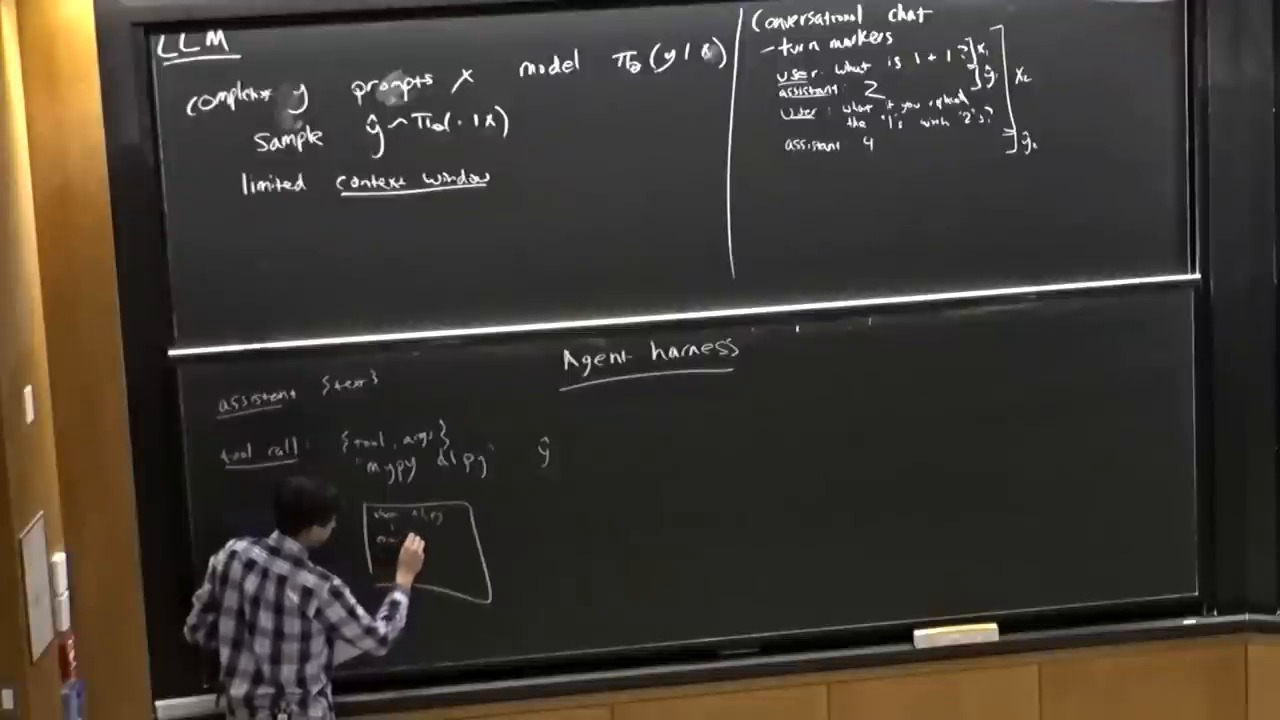
\includegraphics[width=0.92\textwidth]{figures/fig_08_tool_board.jpg}
\caption{模型的输出可以是一个工具调用请求，例如运行 mypy dl.py\vtag}
\end{figure}
\srcnote{00:19:00--00:19:15}
\end{minipage}


再加一个想法：既然加了轮次标记，还可以对模型的输出做特殊解释。模型可以输出“助手：一些文字”，也可以输出“调用工具”。也就是训练语言模型，使它能输出在你机器上做事的请求，比如请求运行 \texttt{mypy dl.py}。然后有一段代码包住语言模型，就像对话应用把整个消息历史拼起来构建后续输入一样，这里有一个智能体框架，有时也叫脚手架（scaffolding），它解释模型的这些输出，真的在机器上执行，再把结果作为后续输入送回语言模型。比如 mypy 输出“第 1 行出错，期望 int……”，就把这些输出原样塞进下一次输入，成为送给模型的 $x$ 的一部分。

\noindent\begin{minipage}{\textwidth}
\begin{figure}[H]
\centering
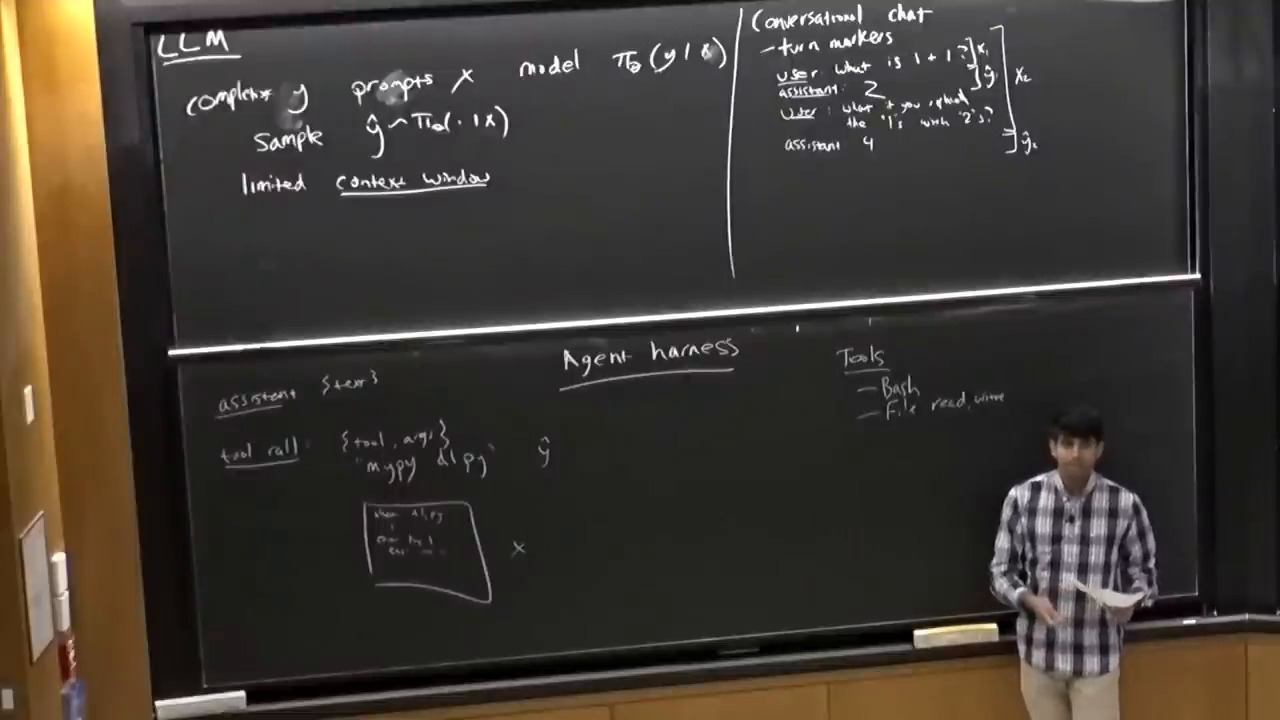
\includegraphics[width=0.92\textwidth]{figures/fig_09_harness_board.jpg}
\caption{智能体框架循环调用模型、执行工具并回传结果，直到模型输出给用户的文字\vtag}
\end{figure}
\srcnote{00:21:00--00:21:15}
\end{minipage}


有同学问智能体框架到底是什么。讲者说它做好几件事：实现循环调用语言模型的那部分代码，拿到输出；如果有工具调用，就分派执行，真的在你机器上运行，拿到产生的文本，回传给语言模型，让它继续。大致是：接收用户输入，然后在循环里调用模型；如果模型请求工具调用，就执行工具，把结果送回模型，生成下一个补全；如果又是工具调用，再执行、再回传……直到模型输出给用户的文字，这时它说“好了，我做完了”，控制权回到用户。工具实现包括 bash（于是可以运行测试、看到测试结果，并据此决定之后的行动）、读写文件等。

\begin{lstlisting}[language=Python]
def agent(user_input, tools):
    history = [("user", user_input)]
    while True:
        y = sample_llm(history)          # y ~ pi_theta(y | x)
        history.append(("assistant", y))
        if is_tool_call(y):
            result = tools.run(y)        # e.g. bash, read_file, write_file
            history.append(("tool", result))
        else:
            return y                     # text for the user; control returns
\end{lstlisting}

\begin{warningbox}{伪代码说明}
讲义作者提醒：上面的伪代码是根据讲者在黑板上的描述整理的示意，真实的智能体框架还要处理权限确认、流式输出、上下文长度管理、错误重试等大量细节。
\end{warningbox}

讲者总结：核心原语就是这些，中心是一个对字符串或 token 的概率分布建模的语言模型，外面是一个循环调用模型、反复采样并分派工具执行、把结果回传以推动任务前进的智能体框架。你输入一个请求时，底层通常会运行一堆工具，多次从语言模型采样。

有同学问框架和模型之间是否有公认的接口，使它们可以互换。讲者说有一些常用接口，虽然没有完全标准化，但如今互通性不错，比如有 OpenCode 这样的开源智能体框架，可以搭配不同的底层模型，Anthropic 的、OpenAI 的等等。又有同学指出语言模型是概率性的。讲者说是的，它是在采样输出字符串并据此行动；模型以聪明的方式训练，但并不像人那样有智能，有时会输出不太对的东西，比如调用你电脑上不存在的命令，或者用读写文件的工具写出错误的代码。但实践中它们效果相当不错，用多了就会建立起对它们擅长什么的直觉。

\subsection{回看演示中的循环}

\noindent\begin{minipage}{\textwidth}
\begin{figure}[H]
\centering
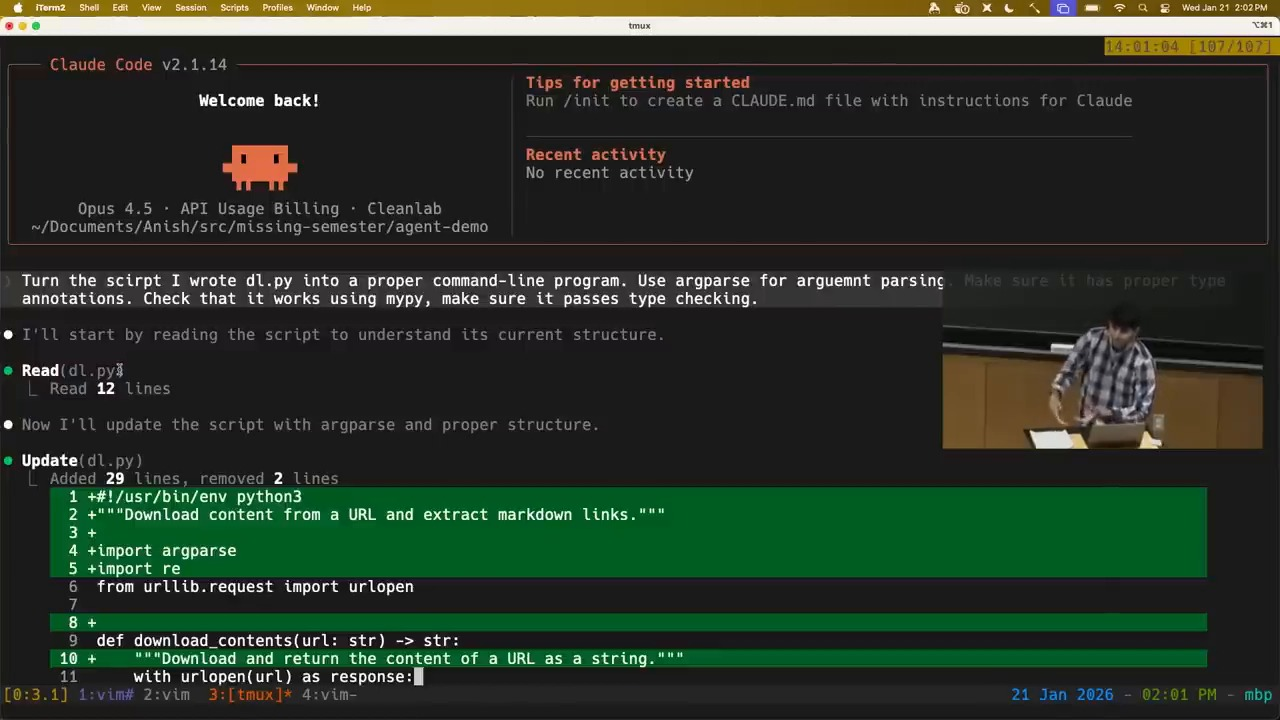
\includegraphics[width=0.92\textwidth]{figures/fig_10_trace_read.jpg}
\caption{回看演示：模型先调用读文件工具读取 dl.py，再输出差异调用写文件工具\vtag}
\end{figure}
\srcnote{00:24:30--00:24:45}
\end{minipage}


讲者把刚才的演示与黑板上的概念对应起来：他用的是 Anthropic 开发的 Claude Code 智能体框架，底层是 Anthropic 的 Opus 4.5 大语言模型。他给出了第一个请求，也就是右上角的初始用户输入；模型输出了一些中间文字，然后决定调用工具：以 \texttt{dl.py} 为参数调用读文件工具。这个请求到了智能体框架，框架把模型输出解释为“模型要求调用工具”，真的在文件系统上执行了读文件操作，得到文件内容，作为下一次的输入送给模型。模型推理采样后，输出一些进度说明，并请求调用另一个工具：写文件工具。在这个框架中（讲者说这也相当常见），写文件工具有几种接口，模型可以提供一个差异，由框架应用到文件上；模型输出的差异也只是一段文本。如此往复，最后是给用户的文字，控制权回到用户。对一个用户请求，内部发生了一大串模型推理步骤和工具调用。

\begin{warningbox}{隐私}
讲者顺带提到隐私：能力更强、更擅长复杂任务的模型需要相当强的硬件来推理，所以基本都在云端运行。使用它们时，除非与服务商有特殊协议，你就是在把数据发给他们，他们可能用这些数据训练等等。如果在意隐私，要仔细看服务条款，或者找到适合自己的方案。
\end{warningbox}

有同学问 Claude 是指模型还是框架。讲者说有几种不同的组合：在这个例子里，框架是 Claude Code，模型是 Claude 系列中的 Opus；但框架和模型可以分开搭配。

\section{用例}

\subsection{开放式的修改}

\noindent\begin{minipage}{\textwidth}
\begin{figure}[H]
\centering
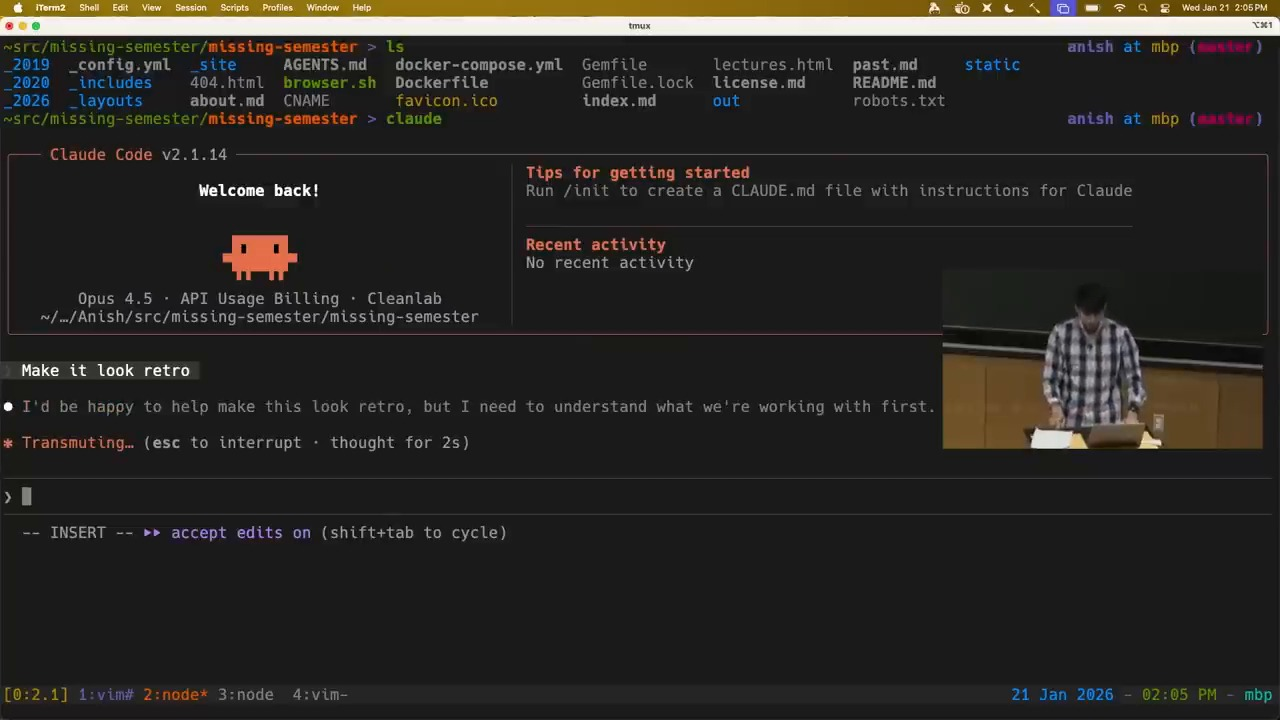
\includegraphics[width=0.92\textwidth]{figures/fig_11_retro_prompt.jpg}
\caption{在课程网站仓库中启动 Claude，只输入一句 make it look retro\vtag}
\end{figure}
\srcnote{00:28:15--00:28:30}
\end{minipage}


讲者说，给这些工具指令时可以非常具体，也可以很开放，再从那里迭代。比如他进入课程网站的 Git 仓库，启动 Claude，只说一句“让它看起来复古一点”，这要一两分钟，先放着回头再看。

\subsection{根据失败的测试修复 bug}

\noindent\begin{minipage}{\textwidth}
\begin{figure}[H]
\centering
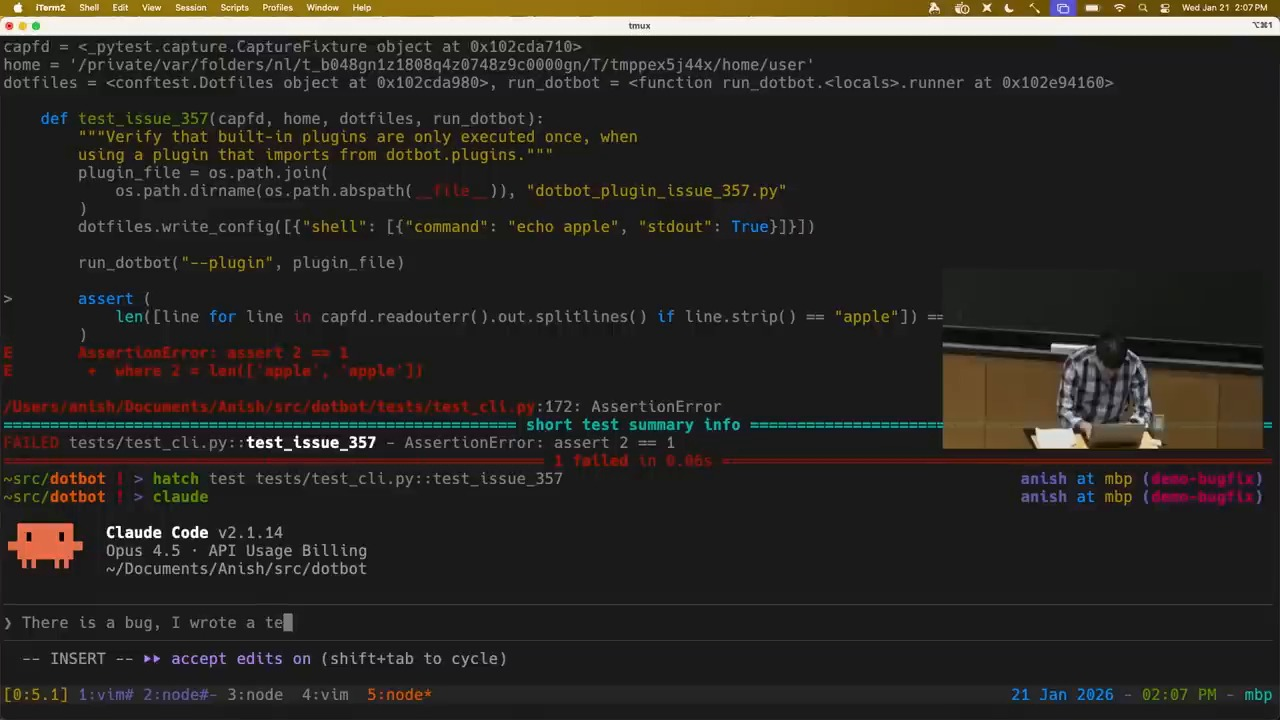
\includegraphics[width=0.92\textwidth]{figures/fig_12_bugfix_test.jpg}
\caption{先运行手写的单元测试复现 bug，确认它确实失败\vtag}
\end{figure}
\srcnote{00:30:00--00:30:15}
\end{minipage}


编码智能体另一个很好的用途是修复代码中的问题：编译不过、linter 报错（周五会细讲 linter）、测试失败。讲者说演示起来有点难，因为想在真实代码库中做，而大家不了解那个代码库，所以不用在意细节，看高层流程就好。他发现代码里有个问题，并为它手写了一个单元测试，运行测试，确实失败了。

他告诉智能体：有个 bug，我为它写了一个测试，用这个命令运行可以复现，修好它。智能体就像人类开发者那样，先运行测试复现 bug：它用 bash 调用他给的命令运行那个测试，看输出，确认确实失败。

\noindent\begin{minipage}{\textwidth}
\begin{figure}[H]
\centering
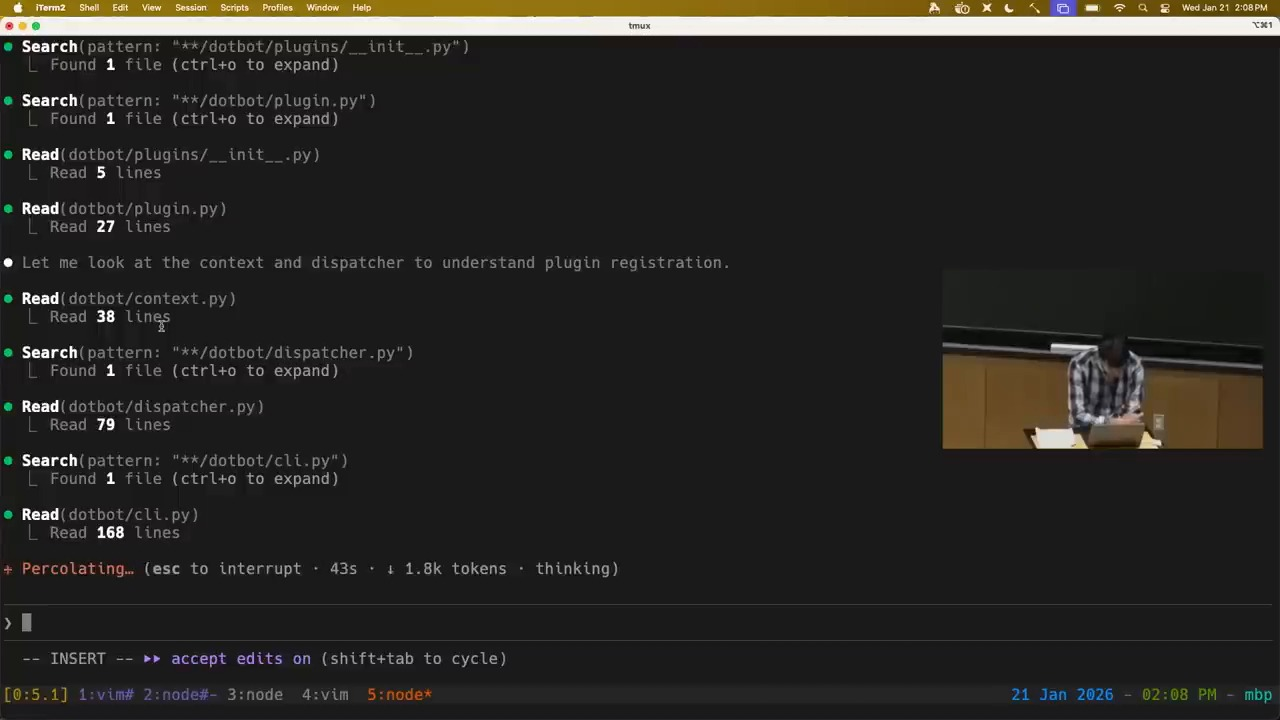
\includegraphics[width=0.92\textwidth]{figures/fig_13_bugfix_search.jpg}
\caption{智能体在代码库中反复搜索和读取相关文件以理解问题\vtag}
\end{figure}
\srcnote{00:31:00--00:31:15}
\end{minipage}


光有失败的输出不足以修 bug，需要真正读懂代码，所以智能体接下来在搜索、阅读、搜索、阅读、思考。讲者说，让这些智能体难以演示的另一个原因是它们不算快，很多人正在研究怎样让智能体既好又快；这个已经跑了整整一分钟，而他想做现场演示，没法快进。这个 bug 足够简单，应该能一次修好。修好之后它还运行了其余测试，确保没有破坏代码库的其他部分。

\noindent\begin{minipage}{\textwidth}
\begin{figure}[H]
\centering
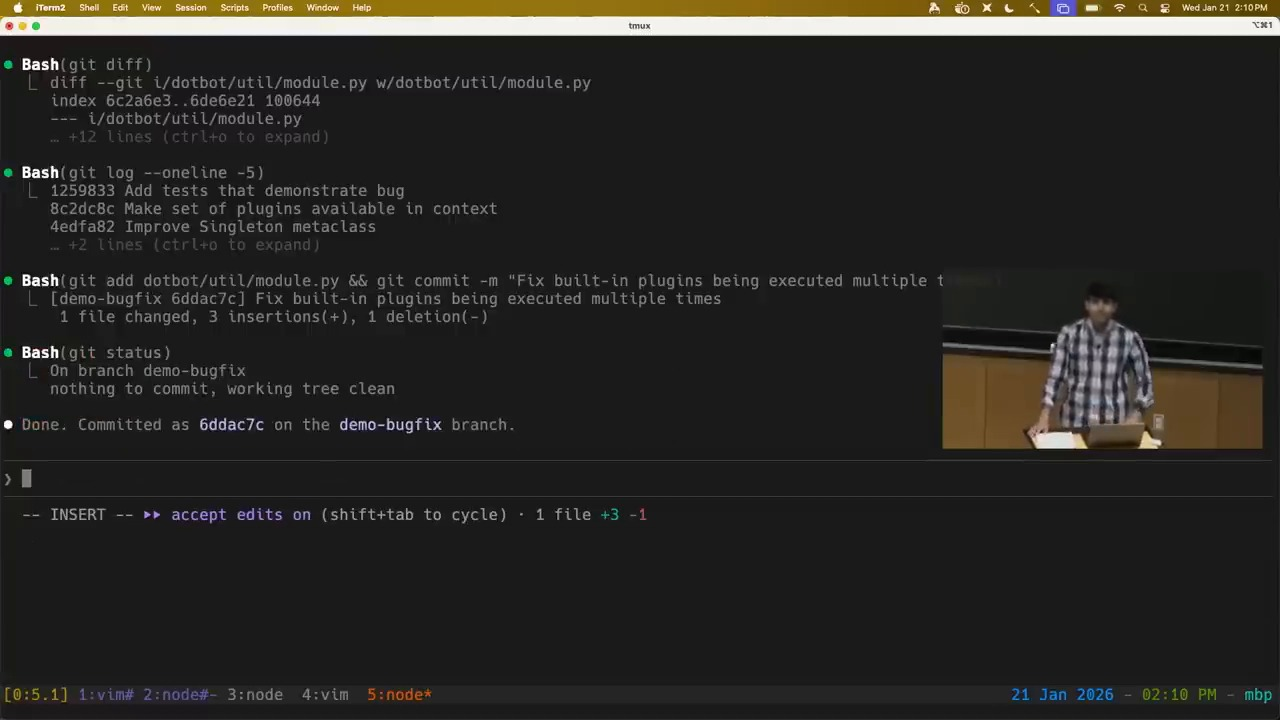
\includegraphics[width=0.92\textwidth]{figures/fig_14_commit.jpg}
\caption{修复完成后让智能体提交，它参照仓库已有风格写出提交信息\vtag}
\end{figure}
\srcnote{00:33:00--00:33:15}
\end{minipage}


完成后，智能体给出了修改总结。讲者又说“提交这些修改”，它就创建了一个带有用提交信息的 Git 提交。他指出这些模型训练得相当好：它学会了不要随便编一个提交信息，而是遵循仓库的风格，所以会先查看已有的提交记录。

有同学问给智能体的提示词和底层模型是否影响代码质量、代码冗长程度、完成任务的时间等。讲者说绝对会，目前写好提示词更像艺术而非科学；而且底层模型在不断改进，两年前的老模型也许也能完成这样的任务，但你得非常详细地描述怎么做，而现在只要简单描述就行。网上有很多资源讲怎样有效地提示这些工具完成各类任务，比如怎样让它实现一个复杂功能。像“让它复古一点”这种小事一句话就够；但对复杂、严肃的功能，提示词可能有好几段长；或者你想更接近工业界的软件开发实践，戴上产品设计师和产品经理的帽子，先写一份完整的设计文档。

又有同学问智能体能否看到目录及其子目录中的一切。讲者说大体上是的，有些智能体还能请求查看目录外的东西，各工具细节不同，但一般应该在 Git 仓库的层面上操作。

\noindent\begin{minipage}{\textwidth}
\begin{figure}[H]
\centering
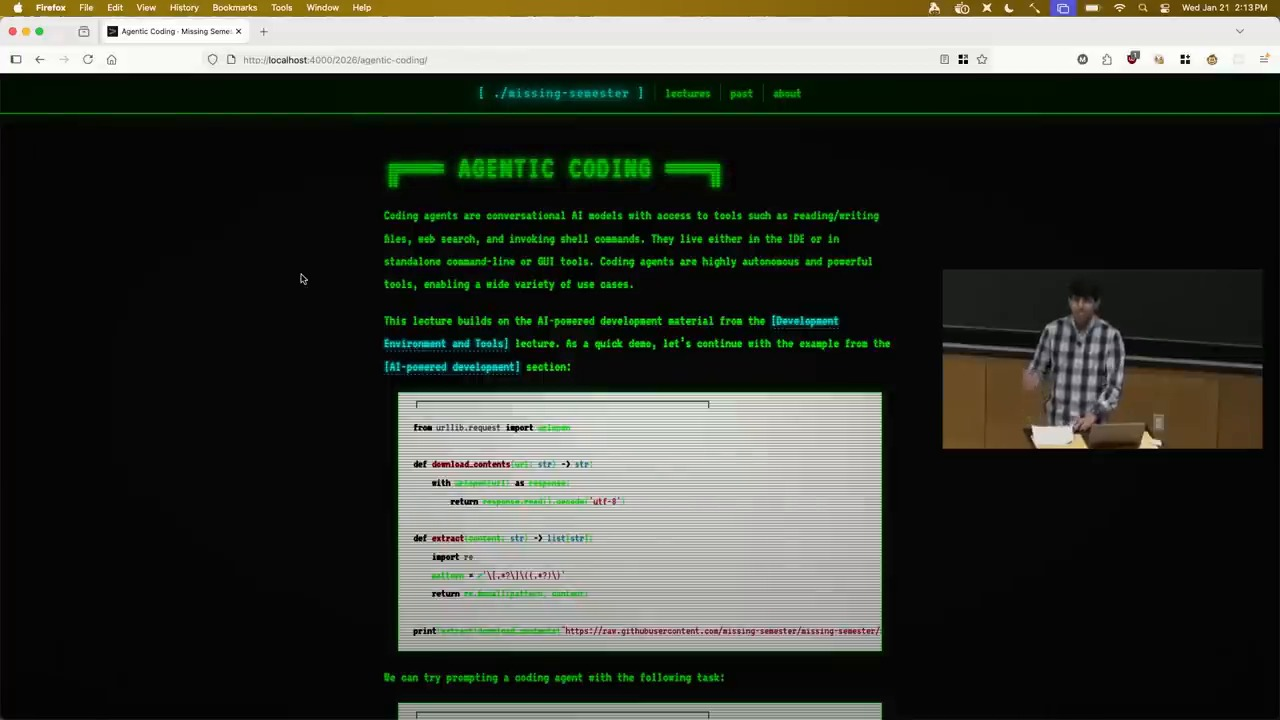
\includegraphics[width=0.92\textwidth]{figures/fig_15_retro_site.jpg}
\caption{复古风格的课程网站：黑底绿字、终端风格的页面\vtag}
\end{figure}
\srcnote{00:36:00--00:36:15}
\end{minipage}


回头看“复古”任务，它已经完成了，讲者说就不提交推送了。他还提到，课程网站的讲义本身就是用 Claude Code 重构的：效果不错但不完美，没有把所有习题搬过去放对位置，有些消失了，他得手动恢复，可以看那个 GitHub 拉取请求了解智能体做了什么、他事后手动修了什么；网站上的 Tufte 风格旁注也是用 Claude Code 实现的，讲者说 Jon 一行代码都没自己写，全是和 Claude Code “氛围编程”出来的。

\subsection{更多用例}

讲者简要介绍了讲义中列出的其他用例，并说大家肯定能想出更多：
\begin{itemize}
\item 重构：他们用 Claude Code 重构了讲义，同样可以重构代码；
\item 代码审查：别人发来 GitHub 拉取请求，或者只是想审查自己的修改，都可以让智能体审查。讲者说智能体相当擅长推理代码和代码之间的差异，曾经指出“你做了这个修改，在这种情况下行为其实不同了”，他据此修了一个 bug；
\item 理解代码库：听众中不少人刚开始学计算机，可能在做较小的仓库；如果想为 GitHub 上的开源项目做贡献，或者深入一个大型代码库，可以让智能体帮你理解它；
\item 当作 Shell 使用：记住 Shell 命令和各种参数可能很难，讲者如今就这样用。
\end{itemize}

\noindent\begin{minipage}{\textwidth}
\begin{figure}[H]
\centering
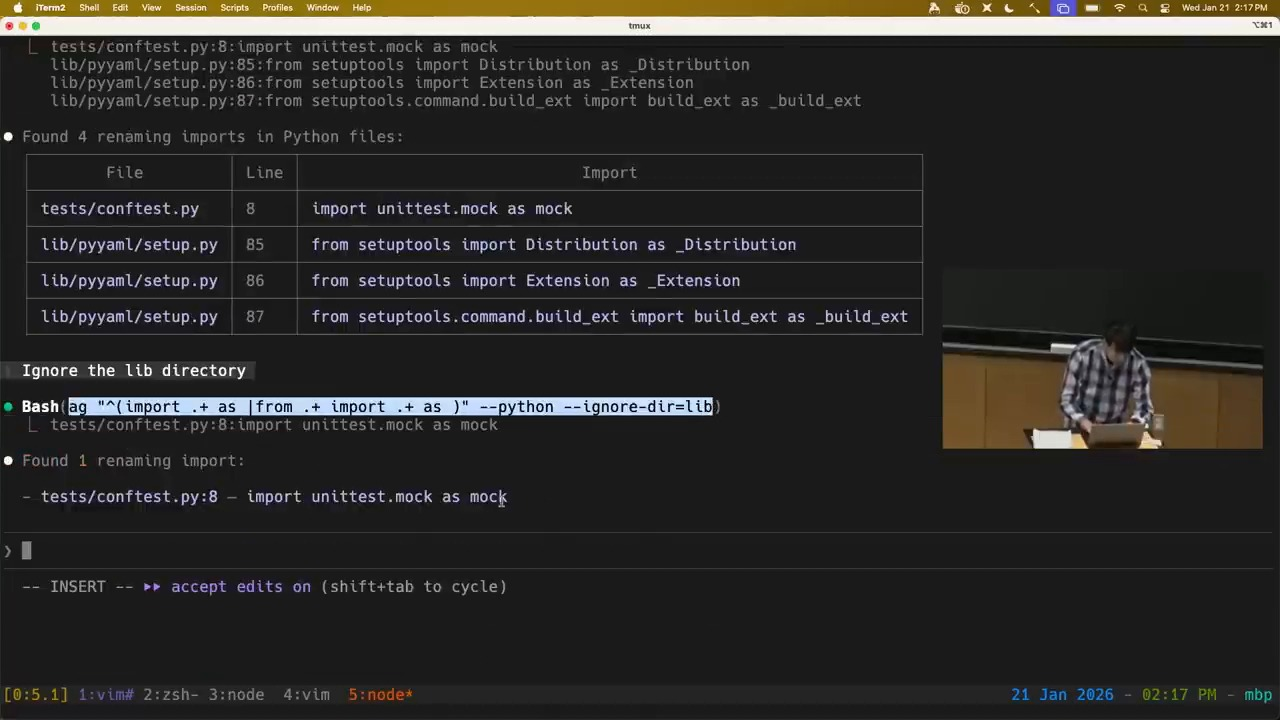
\includegraphics[width=0.92\textwidth]{figures/fig_16_ag_search.jpg}
\caption{让智能体用 ag 找出所有使用重命名导入的 Python 文件，它生成命令并汇总结果\vtag}
\end{figure}
\srcnote{00:40:00--00:40:15}
\end{minipage}


比如他想找出当前目录中所有使用重命名导入的 Python 文件，即 \texttt{from x import y as z} 或 \texttt{import x as y} 这种模式，就说“用 ag 找出所有做重命名导入的 Python 文件”。它生成了正确的 Shell 命令，运行并汇总了结果；结果里包括虚拟环境中的文件，他追加一句“只搜我写的代码”，它就调整了。

\subsection{在课程中使用 AI}

有同学问在课业上用这些工具会不会惹麻烦。讲者说请问你的授课老师是否允许，这因课而异：他见过有的课禁止任何 AI 编码工具，连自动补全、行内聊天这些上一讲讲的简单功能都不行，更别说编码智能体；也见过其他课允许使用。如果你想优先保证自己的理解，可以让工具给提示：即使没有专门模式，也可以说“代码里有个 bug，别告诉我是什么，给我指个方向”，效果还可以，可以把它当作替补助教。

最后讲者提到氛围编程（vibe coding）：这些工具很强大，你可以只用英语和模型聊天，从头到尾实现整个项目而不写一个字符的代码。他说今天不深入讲这个。

\section{进阶功能：复用、并行与外部工具}

\noindent\begin{minipage}{\textwidth}
\begin{figure}[H]
\centering
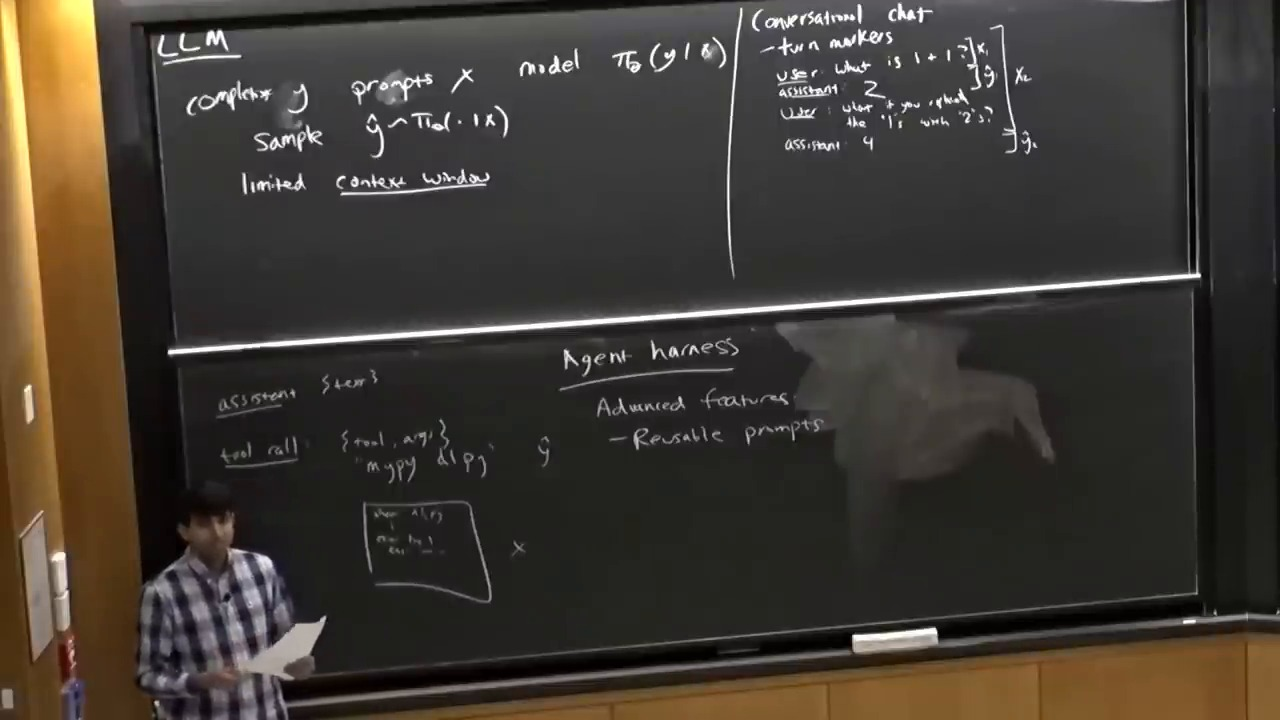
\includegraphics[width=0.92\textwidth]{figures/fig_17_advanced_board.jpg}
\caption{黑板上列出的进阶功能：可复用提示词、并行智能体、MCP 与上下文管理\vtag}
\end{figure}
\srcnote{00:43:00--00:43:15}
\end{minipage}


讲者说最后一部分讲进阶话题，并把它们与前面讲的底层原理联系起来，把要点写在黑板上，从最简单的开始。

\subsection{可复用提示词}

你可能经常给智能体输入同样的指令。比如在某个项目中，你对审查别人发来的拉取请求有特定要求：“这是项目规范，审查要关注代码质量和正确性，但不必担心安全……”你会发现自己经常输入这样的提示词。这些工具通常有功能让你把整段提示词保存下来，之后方便地调用，不用在某个文本文件和智能体之间来回复制粘贴。

\subsection{并行智能体与 git worktree}

\noindent\begin{minipage}{\textwidth}
\begin{figure}[H]
\centering
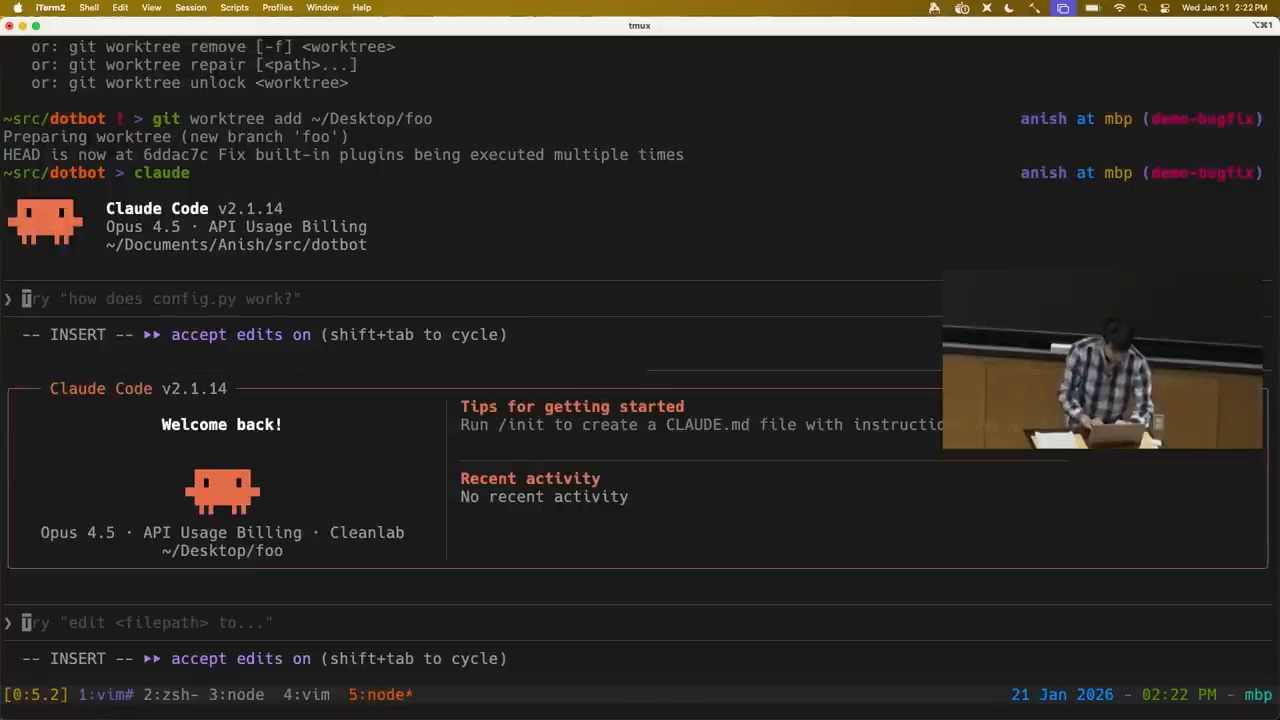
\includegraphics[width=0.92\textwidth]{figures/fig_18_worktree.jpg}
\caption{用 git worktree 创建仓库的另一份独立副本，并在其中启动另一个 Claude\vtag}
\end{figure}
\srcnote{00:45:00--00:45:15}
\end{minipage}


另一个很有用的功能是并行智能体。有些框架内置了这个功能，有些情况下它只是一种工作流。如前面所见，即使相当简单的任务，这些模型也要思考和工作几分钟。如果你想修一个 bug、写一个功能、再写另一个功能，可以并行做。讲者说这节课上他就同时运行着不同的智能体，虽然是在不同仓库：一个 Claude 在把课程网站改复古，另一个在修代码库里的 bug。

在同一代码库上运行多个智能体时，一个非常有用的工具是 git worktree：如果只是在同一个目录里启动多个 Claude 并让它们修改文件，它们会相互冲突；git worktree 让你拥有代码库的完全隔离的副本。他用 \texttt{git worktree add} 创建了仓库的另一份副本，在那里启动另一个 Claude，给它们不同的任务，各自提交到不同分支，完成后再全部合并。讲者说并行智能体和 git worktree 搭配得非常好。

\begin{lstlisting}[language=bash]
git worktree add ../myrepo-feature -b feature
cd ../myrepo-feature
claude
git worktree list
git worktree remove ../myrepo-feature
\end{lstlisting}

\begin{practicebox}{写一个好的任务提示}
讲义作者整理讲者关于提示词的建议：说明目标和验收标准（例如“使这个测试通过，并且不破坏其他测试”）；给出复现或验证的命令；指出相关文件和约束（例如“不要修改公共接口”）；复杂功能先让智能体写计划或设计文档，审阅后再实现。
\end{practicebox}

\subsection{MCP：连接外部工具}

前面有同学问是否有连接框架和模型的标准协议；与此相关，有一个标准化的协议叫模型上下文协议（Model Context Protocol，MCP），用于把智能体框架连接到工具。有各种开源的和托管的实现，比如可以把编码智能体连接到 Notion：把功能规格写在 Notion 里，然后让智能体读取规格、在代码库中实现功能，通过 Notion 的 MCP 连接器就能读写 Notion。这是把编码智能体框架连接到其他工具的一种方式。

\section{上下文管理}

\subsection{清空、回退与压缩}

\noindent\begin{minipage}{\textwidth}
\begin{figure}[H]
\centering
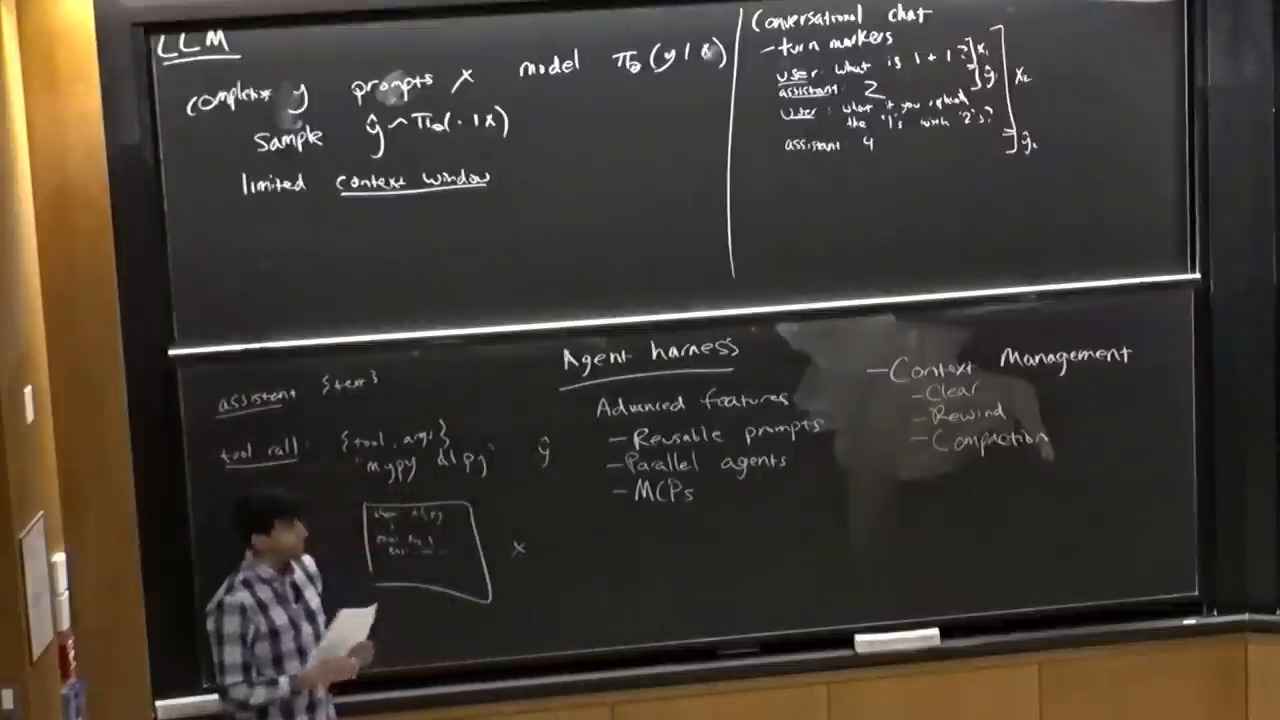
\includegraphics[width=0.92\textwidth]{figures/fig_19_context_board.jpg}
\caption{黑板上的上下文管理：清空、回退、压缩、llms.txt、AGENTS.md、技能与子智能体\vtag}
\end{figure}
\srcnote{00:48:30--00:48:45}
\end{minipage}


接下来是一批与上下文管理相关的功能。回想底层模型的上下文窗口有限：一般模型有固定的窗口，比如只支持最多 100,000 个 token 的输入。实践中，即使技术上在窗口之内，给模型大量输入也会让任务更难，上下文更短、更聚焦时它一般表现更好。

\begin{itemize}
\item 清空上下文：平时聊天时，我们不断往消息历史里追加消息；编码智能体还会把所有工具调用及其输出追加进去，这就是上下文。如果做完一件事想做另一件无关的事，可以结束智能体重新启动，或者用命令清空上下文，从头开始。
\item 回退：有时对话走偏了，比如智能体做错了方向，留着那些内容既混乱又无用。框架一般有命令可以从消息历史末尾弹出消息，回到过去，假装那些事没发生过，把它们从上下文中删除，同样有助于保持上下文较小、模型更专注。
\item 压缩（compaction）：如果底层模型的上下文窗口固定，怎样支持无限长的对话？一般做法是用一个 LLM 把消息历史总结成更短的历史，用总结替换上下文的前缀，于是可以继续对话。在 Claude Code 中可以调用 \texttt{/compact} 命令；这些工具一般会自动压缩，但如果你和智能体聊了很久，上下文长到影响效果，也可以手动调用。
\end{itemize}

有同学问：模型开始压缩时，是让它压缩还是开一个新会话？讲者说这也更像艺术而非科学：如果还在同一条线上继续，LLM 生成的压缩总结相当不错，继续就好；如果要做无关的事，就清空上下文，不要留着一堆没用的上下文，哪怕是总结。

\begin{knowledgebox}{为什么长上下文会变差}
讲义作者补充：讲者提到，即使输入仍在上下文窗口之内，内容越多，模型越难从中找到真正相关的信息，表现往往随之下降；同时每次调用都要重新处理整段上下文，耗时和费用也随长度增加。这就是“上下文越短越聚焦越好”的两层原因。
\end{knowledgebox}

\subsection{知识截止与 llms.txt}

\noindent\begin{minipage}{\textwidth}
\begin{figure}[H]
\centering
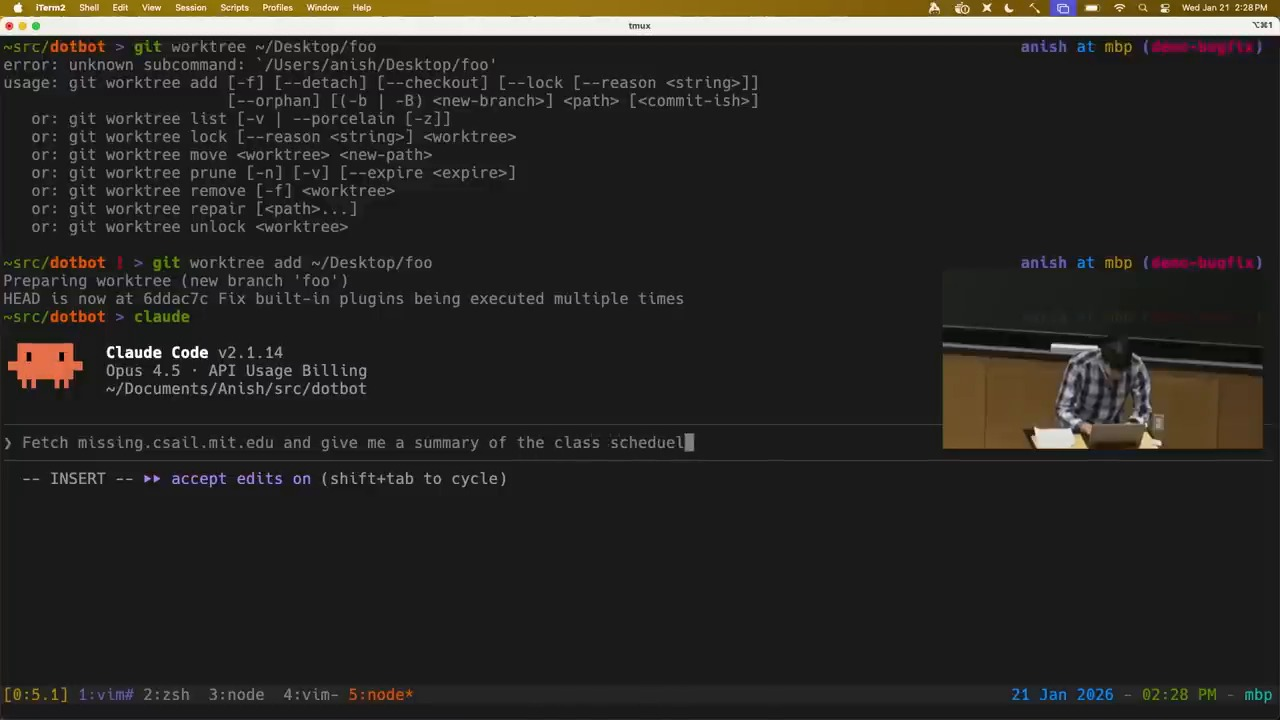
\includegraphics[width=0.92\textwidth]{figures/fig_20_webfetch.jpg}
\caption{让智能体抓取课程网站并总结课程安排，它调用网页抓取工具把内容放进上下文\vtag}
\end{figure}
\srcnote{00:51:00--00:51:15}
\end{minipage}


编码智能体使用的底层模型是冻结的，会不时更新，但在任何时刻都是固定的，用训练时存在的数据训练，不一定了解之后发生的事，这叫知识截止（knowledge cutoff）。如果让智能体用昨天刚发布的库实现功能，模型对这个库一无所知。解决办法是在推理时把信息放进模型的上下文：比如给它库的网址，让它阅读文档，再写代码。编码智能体的工具中有网页抓取工具，它把网页内容取进上下文窗口，然后据此做事。讲者演示了让它抓取课程网站并总结课程安排。

\noindent\begin{minipage}{\textwidth}
\begin{figure}[H]
\centering
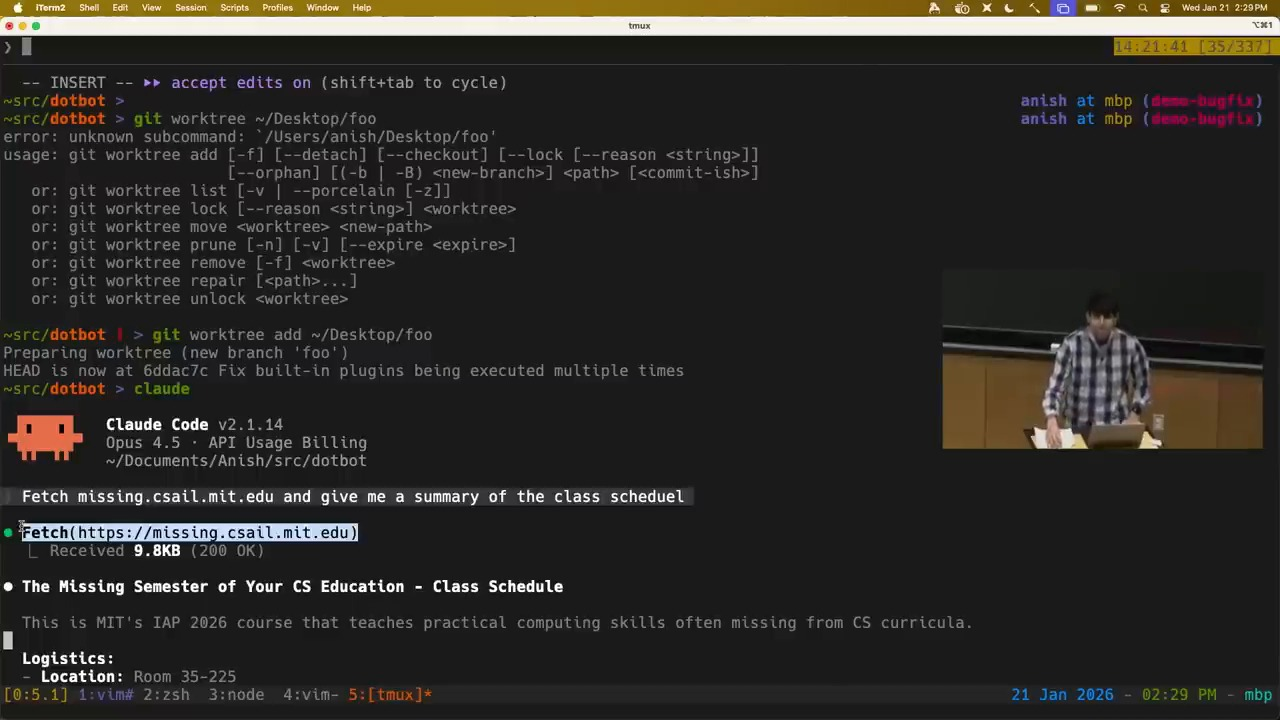
\includegraphics[width=0.92\textwidth]{figures/fig_21_webfetch_result.jpg}
\caption{智能体根据抓取到的页面列出 Missing Semester 2026 的课程安排\vtag}
\end{figure}
\srcnote{00:52:00--00:52:15}
\end{minipage}


llms.txt 就在这里发挥作用：它是一个为 LLM 格式化信息的提议标准。如果把原始 HTML 全部交给智能体和底层模型，HTML 非常冗长，有一大堆与内容无关的东西。很多库，尤其是 AI 相关或比较前沿的，会发布一个 llms.txt。讲者展示了 Pydantic AI 的 llms.txt，比模型抓取 HTML 页面好用得多，尤其是紧凑得多，占用的上下文更少，模型表现也更好。

\subsection{AGENTS.md}

还有一个近乎标准的东西叫 AGENTS.md：放在 Git 仓库或项目中的一个文件，每次启动编码智能体时，它会读取这个文件的全部内容。对 Claude 来说是 CLAUDE.md。课程仓库里就有一个。如果启动时上下文完全为空，智能体对你的仓库一无所知；如果你有特定的实践，比如“运行这个命令做类型检查，运行这个命令跑单元测试”，与其每次都告诉智能体，不如写进这个文件。

\begin{lstlisting}[language=bash]
# AGENTS.md
- Run the type checker with: uv run mypy .
- Run the unit tests with: uv run pytest
- Follow the existing commit message style.
- See docs/STYLE.md before writing documentation.
\end{lstlisting}

\subsection{技能与子智能体}

\noindent\begin{minipage}{\textwidth}
\begin{figure}[H]
\centering
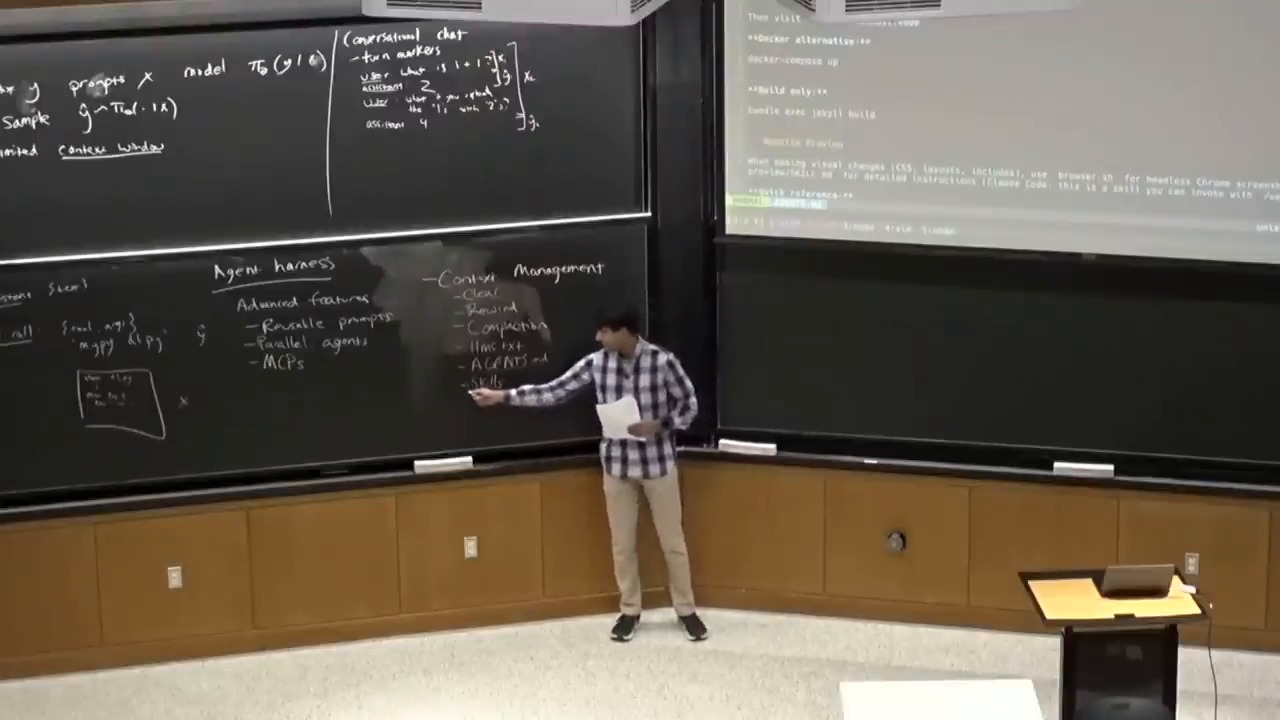
\includegraphics[width=0.92\textwidth]{figures/fig_22_final_board.jpg}
\caption{写满上下文管理要点的黑板，讲者讲到技能与子智能体\vtag}
\end{figure}
\srcnote{00:55:00--00:55:15}
\end{minipage}


另一个与上下文管理有关的概念是技能（skills）。AGENTS.md 先出现，技能可以说是它的后续。人们发现，往 AGENTS.md 里塞大量信息，让智能体一启动就知道项目的一切，很有帮助；但也有缺点：AGENTS.md 很大时，还没开始对话就占掉了上下文窗口的一大块。而且这些文件里往往有很多不同主题的信息，并非每次都需要。于是做法变成：前面只给少量信息，比如“写文档时看这份文档”等等；每个主题的详细信息放在单独的文件里，智能体需要时再打开、按需加载到上下文中，大致相当于一次工具调用。

最后一个上下文管理概念是子智能体（sub-agents）。讲者说：既然有一个智能体，为什么不要多个？部分原因还是上下文管理。如果一个编码智能体在做一个大任务，其中某个子任务需要大量探索，可以派一个子智能体去做，它完成后把控制权交还给父智能体，父智能体的上下文不会被子智能体的细节污染。你可以为编码智能体编写自己的子智能体，它们有时也用于实现智能体的组件：比如有些编码智能体把网页抓取工具实现为子智能体，因为把整个网页的 HTML 加载进模型的上下文窗口不是好主意，子智能体读完网页后只把相关的摘要返回给父智能体。子智能体还能并行：比如你写了一个提示词很好的代码审查子智能体，又写了一个专门修类型检查问题的子智能体，做完一个功能后同时派出两者，Claude Code 就能这样做，它们同时工作，都完成后父智能体继续，这也能提速。讲者说这些功能他只是讲了一遍而没有逐个演示，讲义里有更多细节。

\begin{importantbox}{上下文是稀缺资源}
讲义作者归纳：清空、回退、压缩、llms.txt、技能、子智能体，这些功能背后是同一个原理：模型的上下文窗口有限，而且上下文越短、越相关，模型表现越好。使用智能体时要有意识地管理上下文：任务切换就清空，走偏了就回退，长期知识写进 AGENTS.md，按需知识做成技能，需要大量探索的子任务交给子智能体。
\end{importantbox}

\section{AI 不是魔法}

讲者最后强调：这些工具很强大，但 AI 不是魔法。回到黑板上的定义，语言模型就是一个概率分布 $\pi_\theta$，仅此而已，训练一个好的 $\pi_\theta$ 要用很多巧妙的技术，但 LLM 并不像人那样有智能。所以一定要审查 AI 的任何输出，检查正确性和安全问题。他个人就遇到过很多次：AI 生成的代码乍看合理，却有细微的错误，花了很多时间才找到 bug；有时验证代码甚至比自己写出正确的代码还难。所以对真正关键的东西，他常常自己动手，根本不调用 AI。

\begin{warningbox}{仍然要掌握自己的技能}
讲者说，使用这些工具有很多潜在的缺点需要注意。总的来说，自己具备计算机科学和编程能力仍然很有价值，计算机科学家远没有到被淘汰的地步；但同时，这些工具非常强大，值得学习。他强烈建议大家做这一讲的习题，在实践中学会使用它们。
\end{warningbox}

\begin{practicebox}{练习}
讲义作者整理：选一个自己的小项目，先写一个失败的测试，让编码智能体在需要逐个批准命令的模式下修复它，观察它读了哪些文件、运行了哪些命令；为项目写一个 AGENTS.md，记录运行测试和类型检查的命令，开一个新会话验证智能体是否遵循；用 git worktree 同时让两个智能体处理两个独立的小任务，最后合并。
\end{practicebox}

\section{总结}

\begin{itemize}
\item 编码智能体是对话式 AI 模型加上读写文件、运行命令等工具，能端到端完成编程任务；建议逐个批准有风险的工具调用。
\item 语言模型是条件概率分布 $\pi_\theta(y \mid x)$，上下文窗口有限；多轮对话靠轮次标记拼接历史；智能体框架在循环中采样、执行工具调用、回传结果，直到输出给用户的文字。
\item 典型用例：根据失败的测试修 bug、开放式修改、重构、代码审查、理解代码库、当作 Shell 使用；在课业中使用前先确认课程政策。
\item 进阶功能：可复用提示词、并行智能体与 git worktree、MCP，以及清空、回退、压缩、llms.txt、AGENTS.md、技能、子智能体等上下文管理手段。
\item AI 不是魔法：审查输出，关键代码自己写，保持自己的编程能力。
\end{itemize}

\begin{practicebox}{自测}
\begin{enumerate}
\item 用自己的话描述智能体框架的主循环；什么时候控制权回到用户？
\item 为什么说测试驱动开发与编码智能体特别搭配？
\item 多个智能体在同一个仓库目录里同时工作会出什么问题？git worktree 怎样解决？
\item AGENTS.md 和技能都能给智能体提供项目知识，二者在上下文占用上有何区别？
\item 什么情况下应该清空上下文，什么情况下让它压缩？
\end{enumerate}
\end{practicebox}

\end{document}
